
\documentclass[20pt,usenames,dvipsnames]{beamer}

\usepackage[ngerman,english]{babel}
\usepackage{tikz}
\usepackage[normalem]{ulem}
\geometry{paperwidth=10in, paperheight=7.5in}
\usepackage{animate}
\usepackage{xcolor,colortbl}
\usepackage{booktabs}
\usepackage[utf8]{inputenc}


\usepackage{color}
\definecolor{mygray}{rgb}{0.8,0.8,0.8}
\definecolor{yellow}{rgb}{1,1,0}

\defbeamertemplate{description item}{align left}{\insertdescriptionitem\hfill}
%%	should be the very last package to be loaded
\usepackage{hyperref}

%%%%%%%%%%%%%%%%%%%%%%%%%%%%%%%%%%
%%	Beginning of the document		%%
%%%%%%%%%%%%%%%%%%%%%%%%%%%%%%%%%%
\begin{document}

%%	titlepage - fixed frame:
%%	========================

% \begin{frame}
% 	\titlepage
% \end{frame}
\begin{frame}[plain]
	%\titlepage
	\vspace{-3cm}
 \centerline{\includegraphics[scale=.165]{beamerstrip3.png}}

	
	\huge
	\vspace{1em}
	
	Prevalence and the variance of state occupancy time\\
	\vspace{1em}
	\large 
	Tim Riffe and Iv\'{a}n Williams 
\end{frame}
% %-------------------
\begin{frame}[plain]
 \Huge
 \begin{center}
   \includegraphics[height=\textheight]{Figs/Inputs.pdf}
 \end{center}
\end{frame}
%-------------------
\begin{frame}[plain]
\Huge
\begin{center}
Question: \pause In a Sullivan setting, can we know the variance of state occupancy time?
\end{center}
\end{frame}
%-------------------
% include example of Sullivan inputs:
% l_x and pi_x
%-------------------
\begin{frame}[plain]
\Huge
\begin{center}
Answer: \pause No, sorry. \pause \\ But wait!
\end{center}
\end{frame}
%-------------------

% this could be replaced with series of figures?
% trajectories figure, 2 or 3 steps
% traj -> dist -> var?
\begin{frame}[plain]
\Huge
\begin{center}
Preliminary observations \\
\Large \pause
\begin{itemize}[<+->]
\item life \textcolor{blue}{trajectories} come first
\item observed or \textcolor{blue}{generated}
\item \textcolor{blue}{assumptions} required
\item let's explore some
\end{itemize}
\end{center}
\end{frame}

%-------------------

% show four Bernouli rewards steps from Zarulli & Caswell



% add step for extracting state distribution
\begin{frame}
\begin{center}
\begin{overlayarea}{\textwidth}{\textheight}
    \only<1>{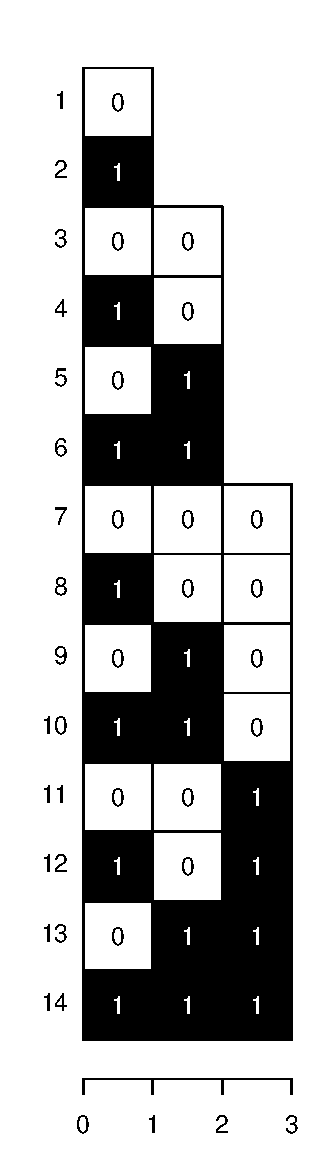
\includegraphics[height=\textheight]{Figs/BernTraj.pdf}}
    \only<2>{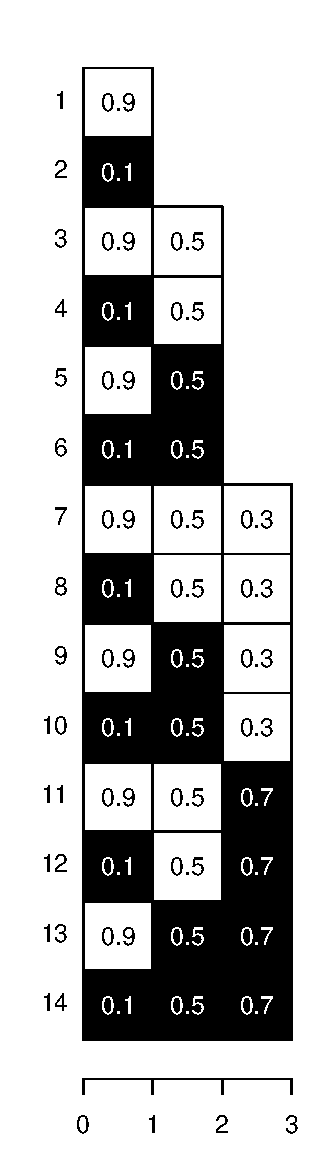
\includegraphics[height=\textheight]{Figs/BernTrajProbs.pdf}}
    \only<3>{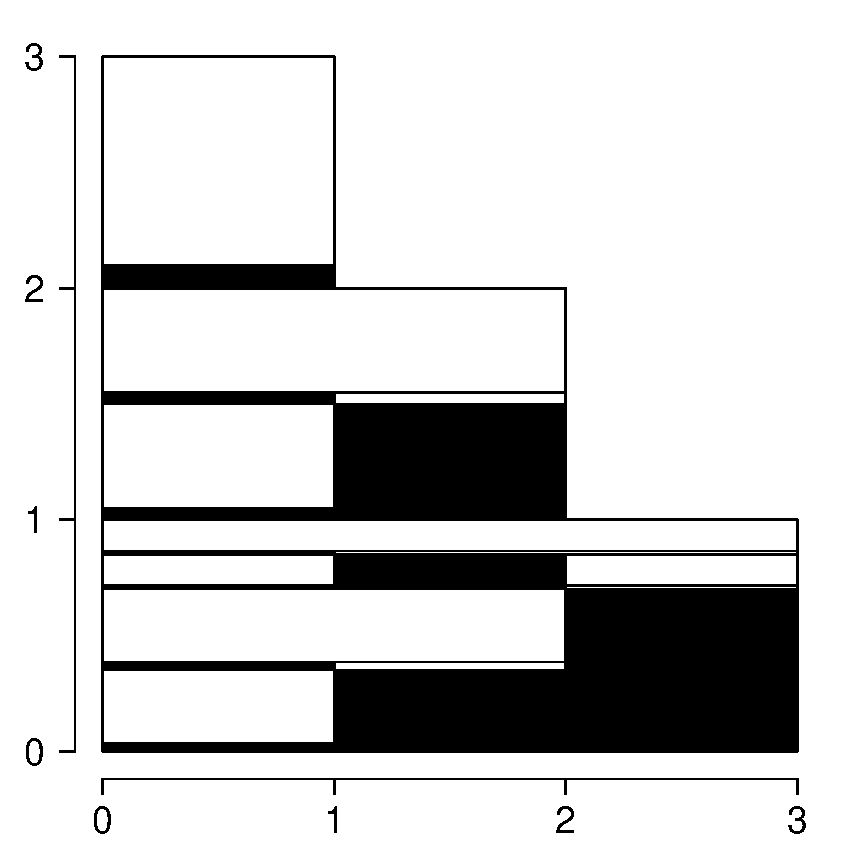
\includegraphics[height=\textheight]{Figs/BernCondTrajProbs.pdf}}
    \only<4>{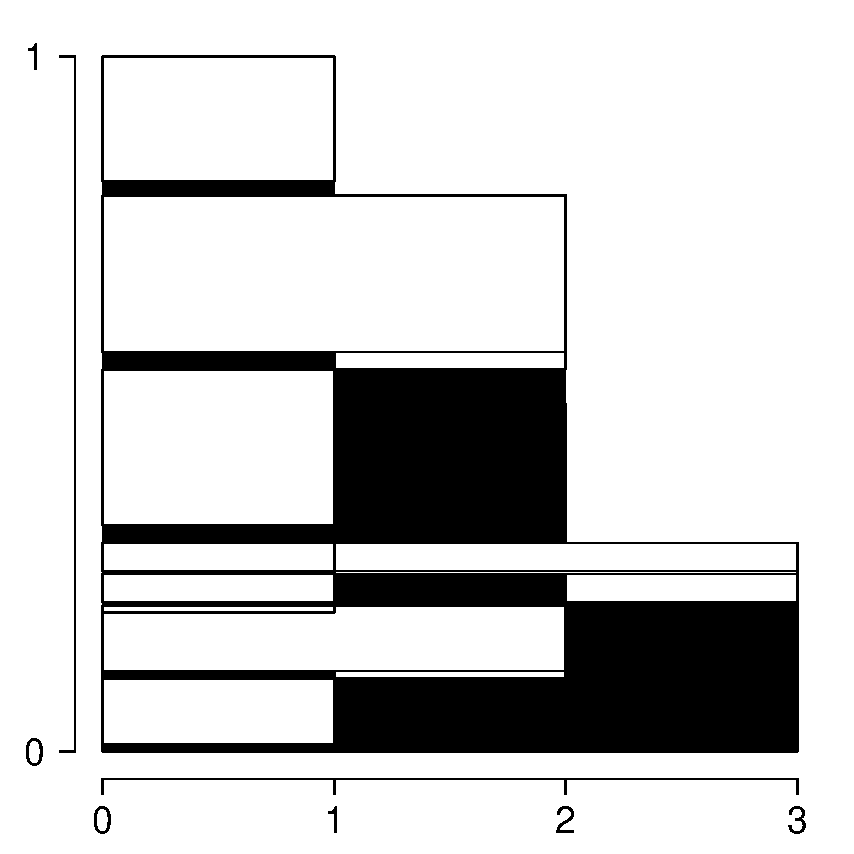
\includegraphics[height=\textheight]{Figs/BernTrajProbsWeighted.pdf}}
    \only<5>{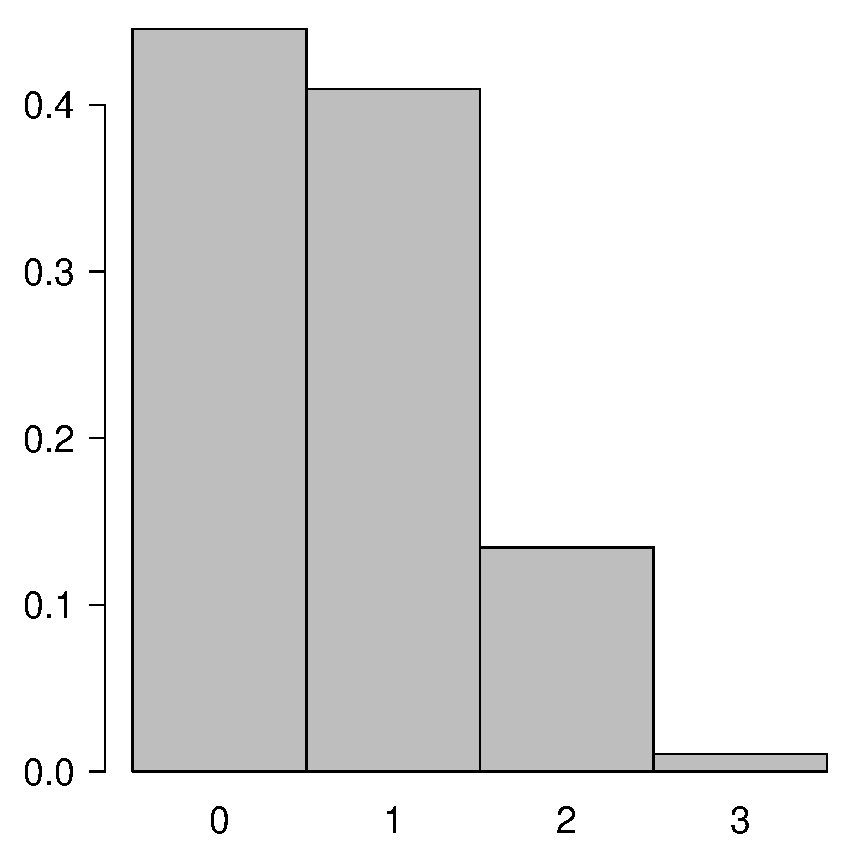
\includegraphics[height=.9\textheight]{Figs/BernDiDist.pdf}}
\end{overlayarea}
\end{center}
\end{frame}
% ------------------

% do same thing for fixed rewards
% 3 steps: 1) bars for fraction of year, 2) jittered. 3) grayscale

% ------------------

\begin{frame}[plain]
\Huge
\begin{center}
Many ways to combine survivorship and prevalence\ldots 
\end{center}
\end{frame}

% ------------------
% random 1,2,3 (pure, tending up, tending down)
% ------------------
\begin{frame}
\begin{overlayarea}{\textwidth}{\textheight}
    \only<1>{\includegraphics[height=\textheight]{Figs/InputsBlocky.pdf}}
    \only<2>{\includegraphics[height=\textheight]{Figs/Bottom1.pdf}}
    \only<3>{\includegraphics[height=\textheight]{Figs/Top1.pdf}}
    \only<4>{\includegraphics[height=\textheight]{Figs/HCAL.jpg}}
    \only<5>{\includegraphics[height=\textheight]{Figs/Min1.pdf}}
    \only<6>{\includegraphics[height=\textheight]{Figs/Random1.pdf}}
    \only<7>{\includegraphics[height=\textheight]{Figs/Random2.pdf}}
    \only<8>{\includegraphics[height=\textheight]{Figs/Random3.pdf}}
    \only<9>{\includegraphics[height=\textheight]{Figs/FixedDecimal.pdf}}
\end{overlayarea}
\end{frame}
% ------------------
% bounds prevalence bottom and top
% ------------------

\begin{frame}[plain]
\Huge
\begin{center}
Anscomb\emph{osaurus}~~\small (HT Alberto Cairo)
% add picture (w trex?)
\includegraphics[width=\textwidth]{Figs/AllDinosGrey.png}
\end{center}
\end{frame}

% ------------------

\begin{frame}[plain]
\Huge
\begin{center}
\emph{Sullivans Sextet} 
% add picture (w trex?)
\includegraphics[height=.9\textheight]{Figs/SullivanSextet.pdf}
\end{center}
\end{frame}

% ------------------

\begin{frame}[plain]
\Huge
Prevalence scenarios
% add picture (w trex?)
\includegraphics[height=.8\textheight]{Figs/Comparison.pdf}
\end{frame}

% ------------------
% and what is reasonable?
% ------------------
% heuristics: TTD prevalence (Klijs), HLETTD lt TTDprev combos
% a more realistic way to fill in lx with prev?
\begin{frame}[plain]
\small
\begin{center}
\includegraphics[height=.8\textheight]{Figs/12889_2011_Article_3213_Fig1_HTML.jpg}
\end{center}

Klijs, Machenback, and Kunst (2011)
\end{frame}

\begin{frame}[plain]
\small
\begin{center}
\includegraphics[height=.9\textheight]{Figs/schematic3.pdf}
\end{center}
Riffe, van Raalte, Bijlsma (2017)\\~
\end{frame}

\begin{frame}[plain]
\huge
\begin{center}
Thanks to:\\
Doug Wolf, Jennifer Karaz Montez, Hal Caswell, Virginia Zarulli,
Alyson van Raalte


\vspace{2em}
\pause
And to you for any comments!\\ \\

\Large
riffe@demogr.mpg.de
\end{center}
\end{frame}
%%%%%%%%%%%%%%%%%%%%%%%%%%%%%%%%%%
%%	End of the document			%%
%%%%%%%%%%%%%%%%%%%%%%%%%%%%%%%%%%
\end{document}






